%%%%%%%%%%%%%%%%%%%%%%%%%%%%%%%%%%%%%%%%%%%
%%% DOCUMENT PREAMBLE %%%
\documentclass[12pt]{report}
\usepackage[english]{babel}
%\usepackage{natbib}
\usepackage{url}
\usepackage[utf8x]{inputenc}
\usepackage{amsmath}
\usepackage{graphicx}
\graphicspath{{images/}}
\usepackage{parskip}
\usepackage{fancyhdr}
\usepackage{vmargin}
\usepackage[T1]{fontenc} % Use 8-bit encoding that has 256 glyphs
\usepackage{booktabs} % for nice lines in tables
\usepackage{color} % text color
\setmarginsrb{3 cm}{2.5 cm}{3 cm}{2.5 cm}{1 cm}{1.5 cm}{1 cm}{1.5 cm}

\title{Applying Reinforcement Learning to Bomberman}								
% Title
\author{Hein-Erik Schnell, Karl Thyssen}						
% Author
\date{\today}
% Date

\makeatletter
\let\thetitle\@title
\let\theauthor\@author
\let\thedate\@date
\makeatother

\pagestyle{fancy}
\fancyhf{}
\rhead{\theauthor}
\lhead{\thetitle}
\cfoot{\thepage}

% displays code within text
\newcommand{\code}[1]{{\fontfamily{pcr}\selectfont #1}}
\newcommand{\state}[1]{$\left\lbrace #1 \right\rbrace$}

% Define command \chapterauthor{author}
\makeatletter
\newcommand{\chapterauthor}[1]{%
	{\parindent0pt\vspace*{-10pt}% Vspace btw heading and author
		\linespread{1.1}\itshape#1 % \itshape is text formatting (italic) 
		\par\nobreak\vspace*{10pt}} % Vspace btw author and text
	\@afterheading%
}
\makeatother


%%%%%%%%%%%%%%%%%%%%%%%%%%%%%%%%%%%%%%%%%%%%
\begin{document}

%%%%%%%%%%%%%%%%%%%%%%%%%%%%%%%%%%%%%%%%%%%%%%%%%%%%%%%%%%%%%%%%%%%%%%%%%%%%%%%%%%%%%%%%%

\begin{titlepage}
	\centering
    \vspace*{0.5 cm}
    
\includegraphics[scale = 0.075]{uni_hd_logo.jpg}\\[1.0 cm]	% University Logo
\begin{center}    \textsc{\Large   Fundamentals of Machine Learning}\\[2.0 cm]	\end{center}% University Name
	\textsc{\Large Final Project  }\\[0.5 cm]				% Course Code
	\rule{\linewidth}{0.2 mm} \\[0.4 cm]
	{ \huge \bfseries \thetitle}\\
	\rule{\linewidth}{0.2 mm} \\[1.5 cm]
	
	\begin{minipage}{0.4\textwidth}
		\begin{flushleft} \large
		%	\emph{Submitted To:}\\
		%	Name\\
          % Affiliation\\
           %contact info\\
			\end{flushleft}
			\end{minipage}~
			\begin{minipage}{0.4\textwidth}
            
			\begin{flushright} \large
			\emph{Submitted By :} \\
			Hein-Erik Schnell\\
			Karl Thyssen  
		\end{flushright}
           
	\end{minipage}\\[2 cm]
	
	%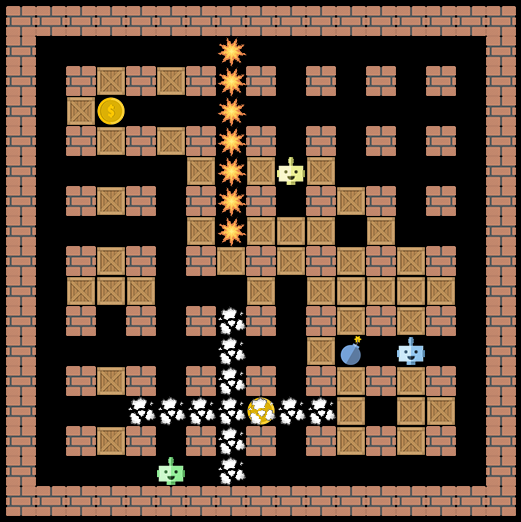
\includegraphics[scale = 0.3]{Bomberman_title.png}
    
    \code{https://github.com/nessyht/FOML-Bomberman}
    
\end{titlepage}

%%%%%%%%%%%%%%%%%%%%%%%%%%%%%%%%%%%%%%%%%%%%%%%%%%%%%%%%%%%%%%%%%%%%%%%%%%%%%%%%%%%%%%%%%

\tableofcontents
\pagebreak

%%%%%%%%%%%%%%%%%%%%%%%%%%%%%%%%%%%%%%%%%%%%%%%%%%%%%%%%%%%%%%%%%%%%%%%%%%%%%%%%%%%%%%%%%
\renewcommand{\thesection}{\arabic{section}}

\section{Learning Method and Regression Model}
\chapterauthor{Hein-Erik Schnell}
This section is divided into the three crucial tasks for which we needed to develop a concept in order to get the agent into training. Those tasks were:

\begin{itemize}
	\item Choosing a suitable \textit{state representation} to be then passed to an \textit{regressor} to estimate the expected \textit{reward} for each of the possible actions
	\item Choosing suitable \textit{rewards} in order to communicate the goals of the game to the agent
	\item Choosing a suitable \textit{regressor} which estimates the expected \textit{reward} for each possible action at the current state of the game.
\end{itemize}

	\subsection{State representation}
	\chapterauthor{Hein-Erik Schnell}
	The first task was to choose a suitable state representation. In case of regressors provided by \textit{scikit-learn}, the training data is usually passed to the regressor as a 2D-array where each row (first index) represents a single state and each column (second index) represents a feature of the respective states. Analagously, the prediction then demands an array of similar form. The regressor then returns an array with as many predicted values as there were rows (states) in the input array. If one wants to predict only a single value, one may not pass a 1D-array to the regressor but create an additional dummy dimension. All this means that if we want to use precoded regressors from scikit-learn, we need to find a 1D-array representation for a single state. \par
	
	After each step, the relevant data is passed to the agent via the dictionary \code{self.game\_state}. In the agents \code{callbacks.py} we defined the function \code{create\_state\_vector(\textit{self})} which turns the information provided by \code{self.game\_state} into a 1D-array. We chose to store the relevant features in the following way:
	
	\subsubsection{State representation 1}
	\label{State_rep_1}
	\begin{itemize}
		\item For each cell:
		\begin{itemize}
			\item \textbf{Agent, Opponent, None \state{1,-1,0}}:\\
			The dictionary provides the entry \code{self.game\_state['arena']} which is a 2D representation of the game board. We use this to create a numpy-array \code{agent\_state} of the same shape which is $1$ on the agents position, $-1$ on cells with an opponent and $0$ on all other cells.
			\item \textbf{Crate, Coin, Empty/Wall \state{-1,1,0}}: \\
			A copy of \code{self.game\_state['arena']} is manipulated in such a way that it is $-1$ for a crate, $1$ for a coin on the respective cell and $0$ in all other cases. This would mean that the agent could not distinguish between empty cells and walls. This issue is resolved later when we delete all cells which contain walls. These cells are always the same and therefore do not contribute to the learning process. In our code, this whole part is represented by the variable \code{loot\_state}.
			\item \textbf{Bombs} \state{6,5 \dots 2,1,0}:\\
			The variable \code{bomb\_state} is of the same shape as \code{self.game\_state['arena']}. All cells are by default $6$. If the cell will soon be affected by a bombs explosion, the values $5\dots2$ represent the 4-time-steps countdown. $1\dots0$ represent the 2-time-steps explosion. This way, \code{bomb\_state} provides a danger level for each cell. $6$ means no danger at all.
			
		\end{itemize}
		\item Just once (implemented in our code as \code{extras}):
		\begin{itemize}
			\item \textbf{Current step number \state{1,\dots,400}}:\\
			\code{extras[0]} contains the current time step.
			\item \textbf{Danger level} \state{0,\dots,6}:\\
			\code{extras[1]} represents the danger level on the agents current position. It is calculated by $6 - \text{\code{bomb\_state[x,y]}}$, where \code{x} and \code{y} are the coordinates of the agents position. Consequently, this danger level in invers to the danger level in \code{bomb\_state}, i.e. $0$ means no danger, $1\dots4$ means increasing danger and $5\dots6$ would be bombs exploding. The least point is rather irrelevant since the agent would already have been deleted by the environment.
			\item \textbf{Bomb action possible \state{0,1}}:\\
			\code{extras[2]} is $1$ if the agent could place a bomb and $0$ if not (i.e. if an own bomb is still ticking).
			\item \textbf{Touching opponent} \state{0,1}:\\
			\code{extras[3]} is $1$ if an opponent is on a neighbouring cell and $0$ if not.
		\end{itemize}
	\end{itemize}

	After manipulating the data in the described way, all cells containing walls are deleted from the 2D-arrays \code{agent\_state}, \code{loot\_state} and \code{bomb\_state}. As already described above, this is done because these entries will always be the same and therefore never contribute to the learning of the agent. The three arrays are then flattened and concatenated after one another into the 1D-array \code{vector}. Finally, we append the \code{extras} to the \code{vector}, which is then returned by the function \code{create\_state\_vector}.\par
	
	With the described representation of a state we combined features which could be represented as seperate features into single features. For example in \cite{paper}, each cell has a feature \textit{Agent on cell?} and \textit{Opponent on cell?} which can both assume the values $0$ and $1$. We combined these two features. As we see it, a proper regressor should be able to determine the important features as well as the relevant range of values of a feature. A \textit{Random Forest Regressor}, for instance, should theoretically be able to do so since the way it works is to find the most relevant feature and its most divisive value.\par
	
	With \textit{state representation 1} ($532$ features), the feature space has at most about $5.4 \times 10^{320}$ possible states. 
	% Calculated with 3^(17*17-34-30-49) * 3^(17*17-34-30-49) * 7^(17*17-34-30-49)*400*7*2*2
	
	\subsubsection{State representation 2}
	\label{State_rep_2}
	As described later in section \ref{results}, our agent never managed to get out of its starting corner. In order to change that, we condensed the above state vector ($532$ features) into a much smaller state vector of $180$ features. The main idea of this smaller state vector is that agents, opponents, crates and coins can never occupy the same cell. Bombs could occupy the same cell as agents, opponents or coins, but for the sake of the agent they shouldn't:
	
	\begin{itemize}
		\item For each cell:
		\begin{itemize}
			\item \textbf{Empty, agent, opponent, crate, coin, danger level} \state{0,1,2,3,4,5 \dots 11}:\\
			Empty cells are $0$. Cells with agent, opponent, crate or coin are \state{1,2,3,4}, respectively. The values \state{5 \dots 11} represent the danger level because there is a bomb affecting the respective cell. $5$ is not used, \state{6 \dots 9} is the four-time-steps countdown, \state{10,11} the two-time-steps explosion. If there is a danger level the values \state{1,2,3,4} are overwritten. This means that the position of the agent might not be represented anymore in this feature.
		\end{itemize}
		\item Just once (implemented in our code as \code{extras})
		\begin{itemize}
			\item \textbf{Danger level} \state{6 \dots 11}:\\ 
			\code{extras[0]} is the danger level at the position of the agent.
			\item \textbf{Bomb action possible} \state{0,1}: \\
			\code{extras[1]} is $1$ if the agent could place a bomb and $0$ if not (i.e. if an own bomb is still ticking).
			\item \textbf{Touching opponent} \state{0,1}: \\
			\code{extras[2]} is $1$ if an opponent is on a neighbouring cell and $0$ if not.
			\item \textbf{Position of agent} \state{18 \dots 271}: \\
			\code{extras[3]} is essentially the enumerated cell number of the agents position. It is calculated by $17x + y$, where $x$ and $y$ are the agents $x$- and $y$-coordinates. 
		\end{itemize} 
	\end{itemize}
	
	With \textit{state representation 2} (180 features) it has at most about $3.4 \times 10^{193}$ possible states, which is much less than with \textit{state representation 1}. For both representations, these are only upper limits. But both are calculated the same way so that these values are useful for comparisons between both representations.
	% Calculated with 12^(17*17-34-30-49) * 6 * 2 * 2 * (17*17-34-30-49)
	
	\subsection{Rewards}
	\chapterauthor{Karl Thyssen}
	The individual rewards for events that occur in a given step contribute to the reward function and are explicitly defined in the \code{reward\_update()} and \code{end\_of\_episode} functions. The other parameter to influence is the discount factor $\gamma$ for the discounted long term reward. We ran training with factors $\gamma = 1.0$ and $\gamma = 0.9$. The reward function is described by a series of \code{if} clauses that determine the quality of the action taken and apply the reward.

\begin{itemize}
	\item \textbf{Valid move}: $-1$ \\Every step is punished in a small way to encourage the agent to complete tasks in the shortest possible time to avoid stacking negative rewards.
	\item \textbf{Wait}: $-5$\\We noticed while running preliminary quick trains that the agent quickly regressed into a pattern of repeated 'Wait's after only a few generations. Arguably other factors were also different at the time so its debatable how effective this now is.
	\item \textbf{Invalid action}: $-100$\\Invalid actions should be punished so the agent quickly learns the connections in between the fields and the restrictions on the frequency of bomb placements.
	\item \textbf{Destroy crate}: $+10$\\The agent should learn to destroy crates.
	\item \textbf{Coin found}: $+20$\\The agent should want to destroy as many crates as possible to find coins.
	\item \textbf{Collect coin}: $+2000$\\The agent is heavily rewarded for finding coins to incentivise coin collection as a primary goal.
	\item \textbf{Killed opponent}: $+10000$\\If the agent does accidentally kill an agent in training it should have a large weighting so this behaviour can be encouraged, particularly as this will be rare initially.
	\item \textbf{Die (from opponent bomb)}: $-2000$\\The agent should learn to avoid all bombs \dots
	\item \textbf{Die (suicide)}: $-1500$\\ \dots but rather die to its own to deny opponents 5 points.
\end{itemize}	
	
	We did not change the rewards in our tweaking due to the fact that we were not sure how to effectively test changes. Our superficial tests (anecdotal) never lead to ground breaking changes and as such we couldn't realistically change them with the expectation that something would be positively influenced. Particularly reflecting the amount of time it would have taken to train even 10 generations of the changes. However, some interesting ideas we would perhaps have next investigated are:
	\begin{itemize}
		\item Whether a movement to a cell should be rewarded based on proximity to other agents/bombs or coins and how we allow these factors to influence the positivity or negativity of an action. I.e. a step towards a coin that is also a step into an exploding bomb should lead to a negative reward.
		\item Should we punish the repetition of actions, such as the movement to a previously occupied cell which may be undesirable and therefore punished with a small negative value, or should this only be the case when not running from a bomb?
		\item Not punishing death or any actions we perceive to be negative but rather only enforce good ones and let the agent decide whether the risks are worth taking that is to say whether the punishment of not getting the reward is discouragement enough.
	\end{itemize}
	
	\subsection{Regressors}
	\chapterauthor{Hein-Erik Schnell}
	In order to estimate the expected rewards properly we need to find a regressor which is both flexible and very decisive with respect to the features. Flexible, because a simple linear regressor would not be able to resemble the volume of states and outcomes. This big variety of possible states, even at the very beginning of an episode, means that many features are not relevant in a given situation. This is the reason why the regressor should also be able to find the most decisive features.\par
	
	Since we will not know whether the competition will be split into two leagues, one for neural networks and one for classical regressors, we initially decided to train both a classical regressor and a neural network and see which one performs better (in its respective league).\par
	
	As a classical model we chose to use a \textit{Random Forest Regressor}. The advantage of this regressor is that it is infinitely flexible can and can cope with whatever shape the reward function may assume. However, it turns out that this regressor is also quite inaccurate and erratic. Its erratic nature might be problematic because the order of the estimated rewards, i.e. which move is the best, is very important. If the order can not be predicted correctly the agent will not choose the best but only a good move. Figure \ref{forest_mlp_comp2} shows how likely this is. We chose to use the Random Forest Regressor provided by \textit{scikit-learn}.\par
	
	As a neural network we chose the \textit{MLP-Regressor} provided by \textit{scikit-learn} mainly for two reasons. The first reason is that we need a precoded regressor since neural networks haven't been subject to the lecture yet. The other reason is that the syntax and available functions of that regressor are the same as for the Random Forest Regressor. This way we only need to change the initialization of our regressor and do not have to change the rest of the code. It is basically changing one line of the code in order to switch between both regressors.\par
	
	The two regressors are initialized as follows:
	\begin{itemize}
		\item \code{RandomForestRegressor()}
		\item \code{MLPRegressor(max\_iter=500)}
	\end{itemize}
	Thus, we used the Forest with its default settings and changed the maximum number of iterations of the MLP to $500$ (default is $200$) because the regressor sent out a warning that $200$ iterations were not sufficient to reach convergence.
	
	\begin{figure}[h]
		\centering
		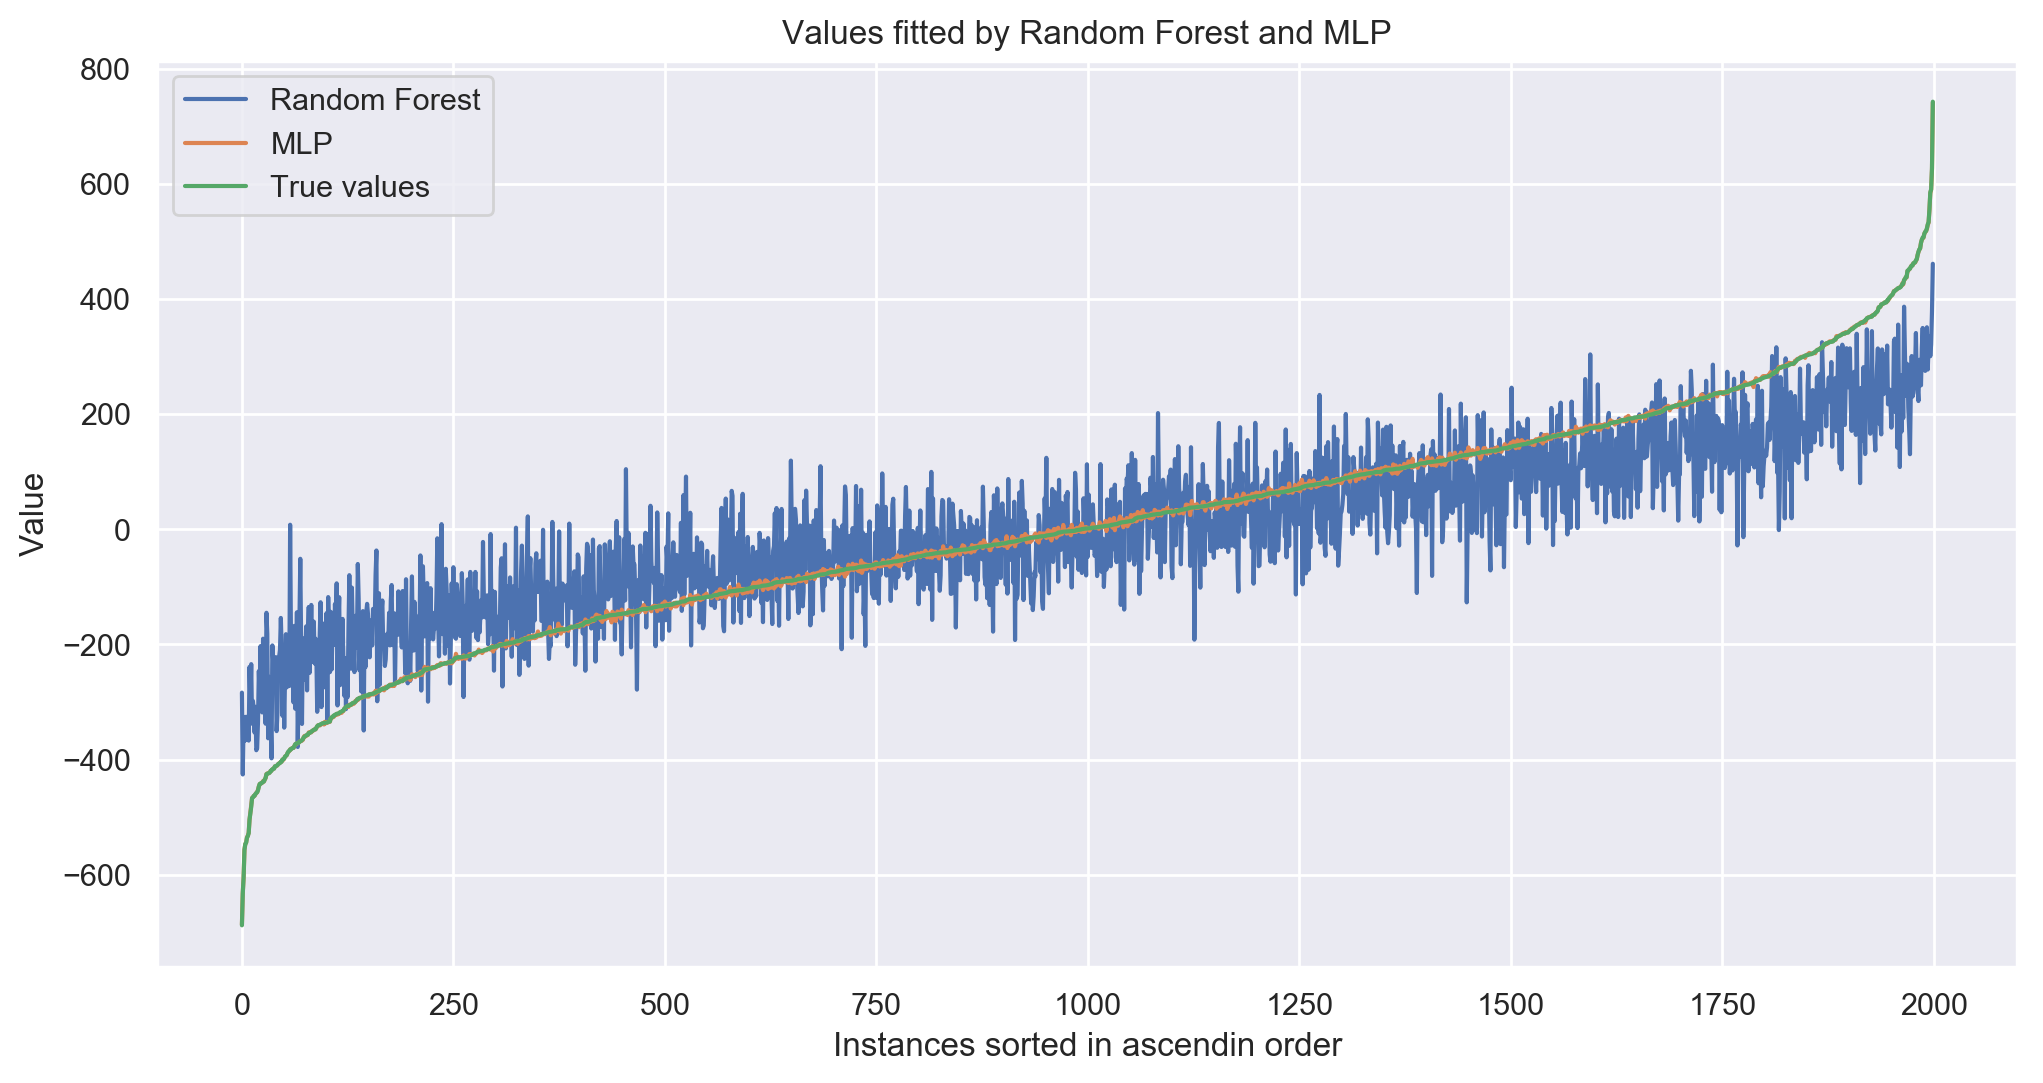
\includegraphics[width=\linewidth]{images/mlp_forest_comparison01.png}
		\caption{\textit{For this figure, {\normalfont \code{sklearn.datasets.make\_regression}} was used to create $10000$ samples with $100$ features of which $10$ are informative. We then trained the Random Forest Regressor and the MLP-Regressor provided by {\normalfont scikit-learn} with $80\%$ of the generated data. The figure shows the predicted values of the remaining $20\%$ of the data which were used as a test set. The test set has previously been sorted by the true target value in ascending order.}}
		\label{forest_mlp_comp1}
	\end{figure}
	\begin{figure}[h]
		\centering
		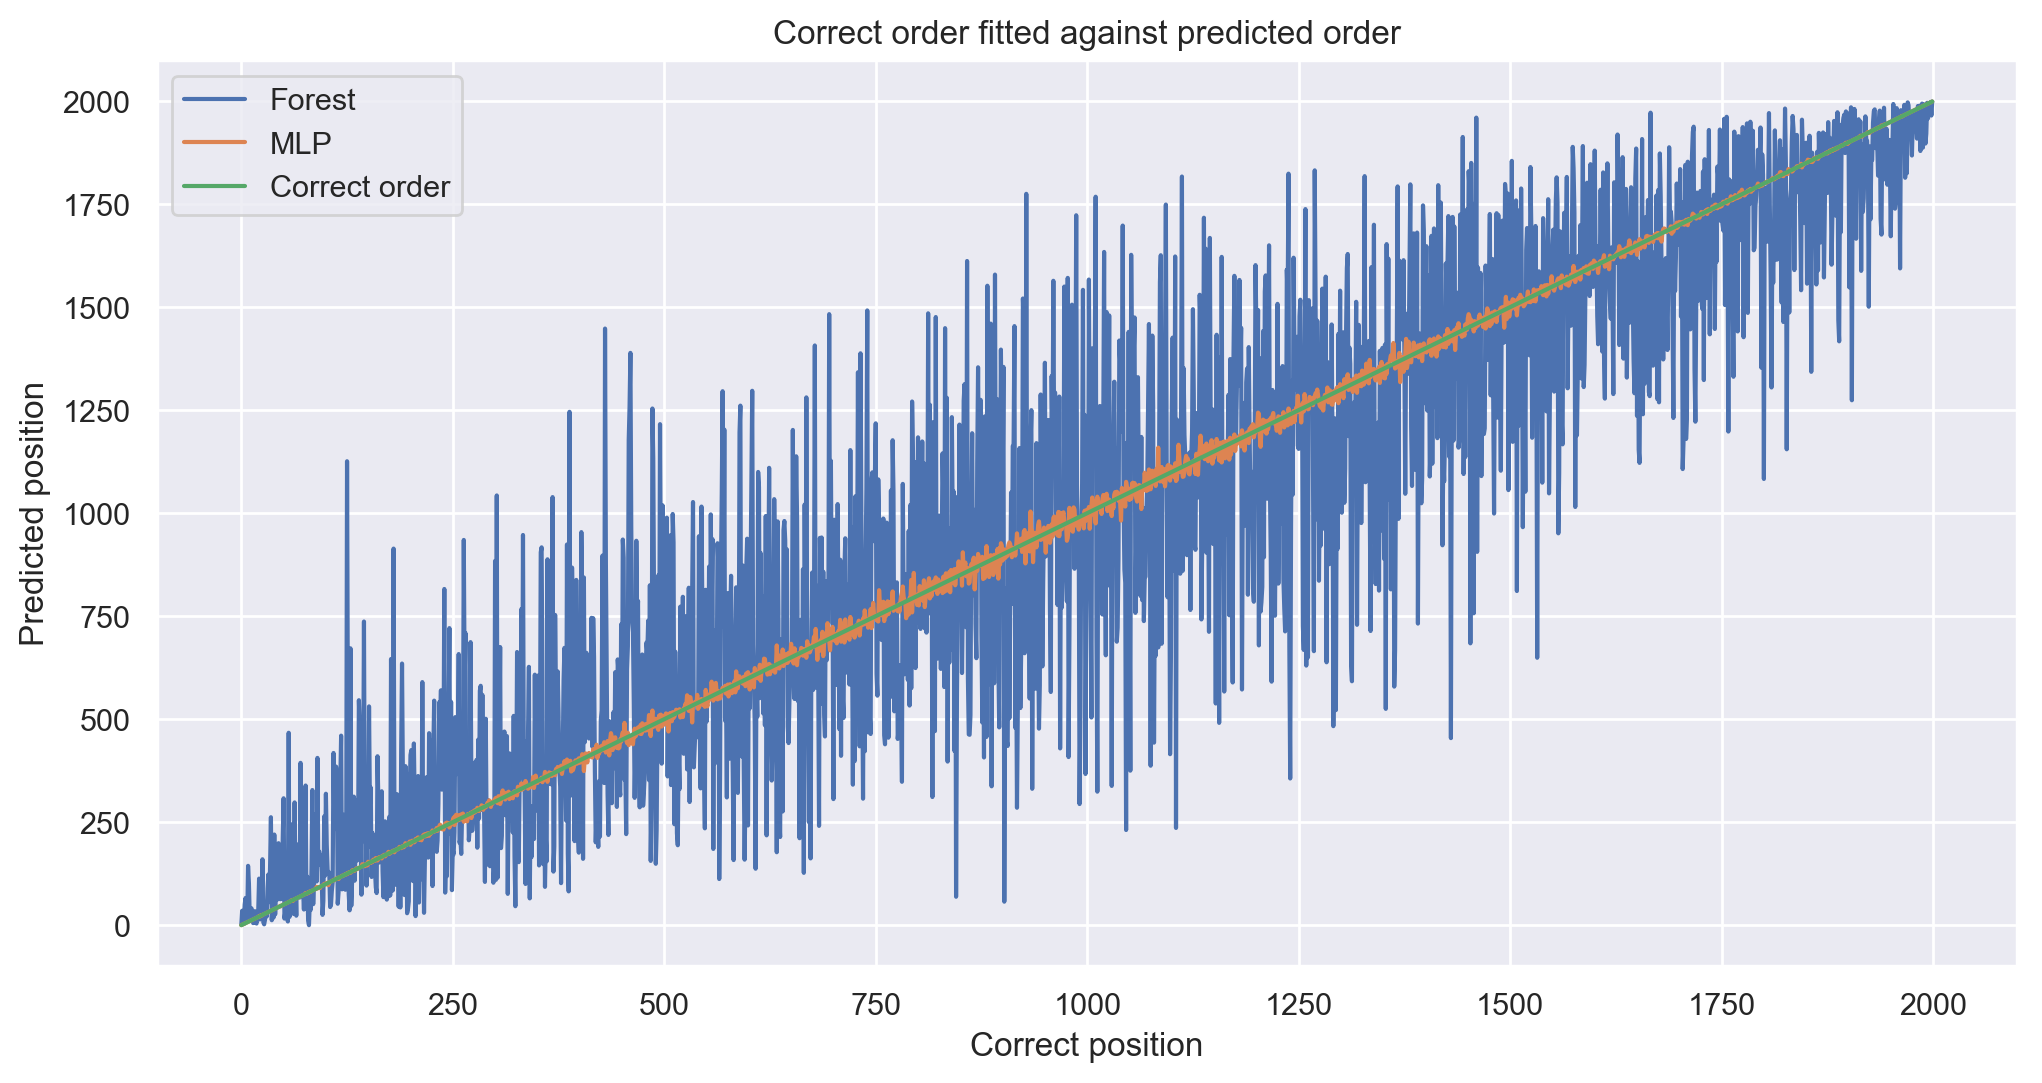
\includegraphics[width=\linewidth]{images/mlp_forest_comparison02.png}
		\caption{\textit{This figure displays the same data as Figure 1. Here, the x-axis represents the position of each instance sorted by its target value, the y-axis displays the position if the instances had been sorted by the predicted target values of the respective regressor. The more the predictions resemble the correct order (the green line) the better the regressor is suited for our task.}}
		\label{forest_mlp_comp2}
	\end{figure}

	In order to get a feeling for the performance of both regressors, we used the function \code{sklearn.datasets.make\_regression} to create $10000$ samples with $100$ features of which $10$ are informative. We then trained the Random Forest Regressor and the MLP-Regressor with $80\%$ of the generated data and let both regressors predict the values of the remaining $20\%$ of the data. Figure \ref{forest_mlp_comp1} shows how much more accurate the MLP-regressor performs compared to the Random Forest Regressor. Figure \ref{forest_mlp_comp2} shows how the MLP-Regressor maintains the order of the instances much better than the Random Forest Regressor. In case of the latter, many values are sorted into completely other regions than where they actually belong. This is also due to the fact that the range of values of the generated data is of the same magnitude as the inaccuracies of the Forest. Still, the MLP manages to predict these values much better.
\newpage
	
	
\section{Training Process}
\chapterauthor{Karl Thyssen}
In reinforcement learning an agent is placed into an environment where it learns to interact with it dependent on the parameters a 'trainer' provides it. Ideally the trainer wishes the agent to embody certain desirable characteristics. This optimal policy is determined by the methodology the trainer uses to reward the agent. Rewards the trainer supplies the agent with are based on the state of the environment at the time the agent is to make a decision and the reward scheme weighting on this given state. 

Initially the agent is often allowed to take random actions to influence the next game-state. This random acting forms the agents initial policy $\pi$. The policy determines how the agent acts in the game, the ideal policy being the ideal way to play the game from the initial game-state.

The rewarding of an agent for a particular action $a$, functions to provide information as to the quality of the decision it made to take this particular action at this particular state $s$; this \state{(state, action)} pair $(s, a)$. Through this feedback the agent can update its policy. Through regular updates of the policy($\pi$), after receiving a reward for games played based on the current policy the agent will begin to favour actions it predicts will lead to higher rewards hence improve the policy and bring it as closely as possible to the optimum.

Formally this is known as the Markov-Decision-Process where the state of the environment at a particular step $t$ in the game is represented as $s_t$ and the action taken for this time step t is represented as $a_t$. The current state is input into the current policy which leads the agent to select its next action. The action is selected from the action space $\mathcal{A} = $\state{\text{UP}, \text{LEFT}, \text{DOWN}, \text{RIGHT}, \text{BOMB}, \text{WAIT}}. The reward for this action $r_t$ is then given by the reward function $r(s_t, a_t)$ given which the agent can then evaluate this move for the update of its policy. In Bomberman its simple to see that the state $s_t$ is given by the distribution of agents, loot, bombs, coins etc. in the game map represented as the trainer wishes. 

In Bomberman an action can not be rewarded entirely isolated from the game as a whole as actions have direct repercussions least 6 steps into the future (by the time the explosion has dissipated) and even beyond. Therefore the action must be rewarded based on all future steps with those very far in the future having decreasing impact. Therefore we introduce a discount factor $\gamma \in [0, 1]$. We arbitrarily selected 0.9 to ensure the steps $n+4, n+5, n+6$ have a non-negligible impact on the reward, as these are the steps that we hope to cash in from a bomb and the agent should see that this was a well placed bomb if this is the case. Unfortunately we see this being very negative as the agent often self-destructs...

Therefore the reward function that the agent is wishing to maximise the expected long term reward $E[\text{Reward}|\pi]$ for the optimal policy is: $$\text{Reward} = \sum_{t=0}^{\infty} \gamma^t r_{t+1}$$. 

The concept of learning refers to the improvement of this policy, by two processes, policy improvement and policy evaluation. As the initial policy in our case will be created by either the random actions of the \code{random\_agent} or the deterministic actions of the \code{simple\_agent}, the initial policy evaluation step will take place on this gathered data.  This is achieved using a value function for each of the states visited in this policy $\pi$. The value function $V$ for each state $s_t$ is the Expected value given the starting state is $s$ of the discounted reward function of the $\pi(a_t|s_t)$ particular pair.

	\subsection{Q-Learning}
	\chapterauthor{Karl Thyssen}
	With our selected state vector of length 532 it would be highly impractical of not impossible to calculate the state action pairs for every state and the expected reward of each action due to the massive amount of data required for this along with the computationally intensive time requirement. Therefore we use the approach of Q-Learning to find the optimal Q function $Q^*$ for each state-action pair in the data, updated using the discounted reward received for the action. We do this in the callback function of the agent when \code{end\_of\_episode()} is called, the discounted rewards are filled into the places of the previously stored immediate rewards of each state-action pair. 
	
	This Q function will need to be updated to find the optimal Q function by gathering data, evaluating the data and updating. To gather data we have 3 options: update Q after every step, after every n-steps or after every n-episodes. Due to the fact that we selected random forest regressors to store our Q the last option seems to suit the purpose best as it is not possible to update sklearn random forest regressors, they must rather be entirely trained from scratch. Therefore it would be incredibly time and storage inefficient to train them on multiple steps, particularly as they will not be effective with small data pools anyway. Therefore we opt to update Q after 10000 as suggested in \cite{paper}.
	
	We store our Q-function as 6 random forest regressors; one for each action, from which the agent will choose an action based on the stochastic policy of the trained forests, each supplying the expected reward for the action it is trained for. This action $a_{t+1} = \pi(a_t|s_t)$ will, in training, be mapped onto the calculated reward along with all state action pairs in the 10,000 games played during each particular policy iteration to retrain the forests, that is to say update the Q-function.
	
	
	\subsection{Exploration and exploitation}
	\label{explo}
	\chapterauthor{Hein-Erik Schnell, Karl Thyssen}
	While optimising the Q function based solely (exploitative approach) on the games of the previous generation (the trees trained on the past $10,000$ games) it is possible to slip into a local maximum in terms of the yield which may well not be the optimal Q. Therefore we introduced a degree of exploration using an $\epsilon$-greedy policy in which a random action is performed with the probability $\epsilon \in [0,1]$. We selected $\epsilon = 0.25$. \par
	
	\subsubsection{Max-Boltzman-exploration}
	When exploration occurs (not the best action is chosen), we decided not to choose the action completely random. Instead, choosing more promising actions should be more likely. This means that the expected rewards need to be mapped onto probabilities with which the respective action is chosen. The probability is given by 
	\begin{align}
		\pi (s,a) = \frac{e^{Q(s,a)/T}}{\sum_{a} e^{Q(s,a)/T}}\text{,}
	\end{align}
	where $\pi (s,a)$ is the probability that the action $a$ is chosen given state $s$, $Q(s,a)$ is the expected reward if action a is performed after state $s$ occured, $a \in \mathcal{A}\setminus a_{max}$ are all available actions after the action with the highest expected reward $a_{max}$ has been deleted from the set of actions $\mathcal{A}$ because $a_{max}$ would have been chosen if we didn't explore, and $T$ is a temperature-parameter which scales the ratios between the probabilities. We found that $T$ should be of about the same magnitude as the expected rewards which is why we chose $T$ as the mean of the absolute values of the expected rewards. Figure \ref{MB_table} shows an example of this.
	\begin{figure}[h]
		\centering
		\begin{tabular}{c|c}
			$Q(s,a)$ & $\pi (s,a)$\\
			\midrule
			$43$ & $0.52$\\
			$21$ & $0.25$\\
			$4$ & $0.14$\\
			$-19$ & $0.07$\\
			$-65$ & $0.02$
		\end{tabular}
	\caption{\textit{Exemplary table of expected rewards $Q(s,a)$ and corresponding probabilities $\pi (s,a)$ if $T$ is chosen as described above. In this case: $T=30.4$}}
	\label{MB_table}
	\end{figure}
	We later decided to enable \textit{exploration} only in one fourth of all rounds. The reason is that the agent can only survive after it placed a bomb if it moves consistently away from it or around a corner. Thus, a random move in every fourth step may be fatal. With the above measure, we could at least ensure the survival after placing a bomb and make the agent learn this behaviour.
	
	\subsection{Training data}
	\chapterauthor{Karl Thyssen}
	We generated new training data after each training generation of $10,000$ games to train the new forests that is to say the Q function for the next generation to learn from. Therefore the size of our final training data array of action state vectors was dependent on the number of rounds the agent survived in a given generation. We saved each set of training data independently of each other to allow for training from any generation and later access to the data. The random forest regressors were also saved to allow for analysis of them and comparison between the generations by allowing play from any generation and even play against younger generation. Ideally play against younger generations would always lead to free wins as the agent should be significantly better after some time, however our agent is a lonely agent that rarely sees others anywhere other than in its state vectors.


\section{Results}
\label{results}
\chapterauthor{Karl Thyssen}
Here we will discuss the results we saw for the various approaches we attempted.

As previously mentioned we experimented with a $\gamma$ value of $1.0$ and $0.9$ after which we continued other variations at $\gamma = 0.9$.
Other variations include:
\begin{itemize}
	\item $\gamma = 1.0$:
	\begin{itemize}
		\item Generation 0 data generated from 4 $\code{simple\_agents}$
		\begin{itemize}
			\item Additionally train MLB
		\end{itemize}
	\end{itemize}
	\item $\gamma = 0.9$:
	\begin{itemize}
		\item Generation 0 data generated from 4 $\code{simple\_agents}$:
		\begin{itemize}
			\item self-train until agents begin to regularly interact with each other
			\item self-train
			\item state vector reduced to 180 elements
		\end{itemize}
		\item Generation 0 data generated from 4 $\code{random\_agents}$:
		\begin{itemize}
			\item self-train until agents begin to regularly interact with each other
			\item self-train
		\end{itemize}
	\end{itemize}
\end{itemize}

%Discuss reasons behind initial approach - also mlp regressor (slow to fit so less data)
\subsection{The initial approach}

Having decided on the random forest regressors as the medium for storing our Q, and knowing the random forest has the ability to determine feature importances and weightings itself we decided to throw every feature we could think at it as described in \ref{State_rep}. We initially also chose a $\gamma$ value of $1.0$ for simplicity in testing and began to train an agent. In \cite{paper} the agent trains for 10000 episodes per generation and begins to show a large improvement between generations $10$ and $20$, however that agent is trained using a neural network so we expected a longer wait before seeing such spikes in performance. This is due to the erratic nature of the predictions made by the forests in relation to the MLP we tested.

Out of interest we also tested the same set-up using an MLP regressor, however unlike the forest, the impact of using any and all features was an exorbitant time required for the fitting after each generation, often longer than the data generation itself.

The average time required to generate data for and fit each generation was roughly $4800 seconds$. This time required is clearly dependent not only on hardware and thinking time but also the number of steps the agent takes per episode which was unfortunately consistently short.

\begin{figure}[h]
\centering
	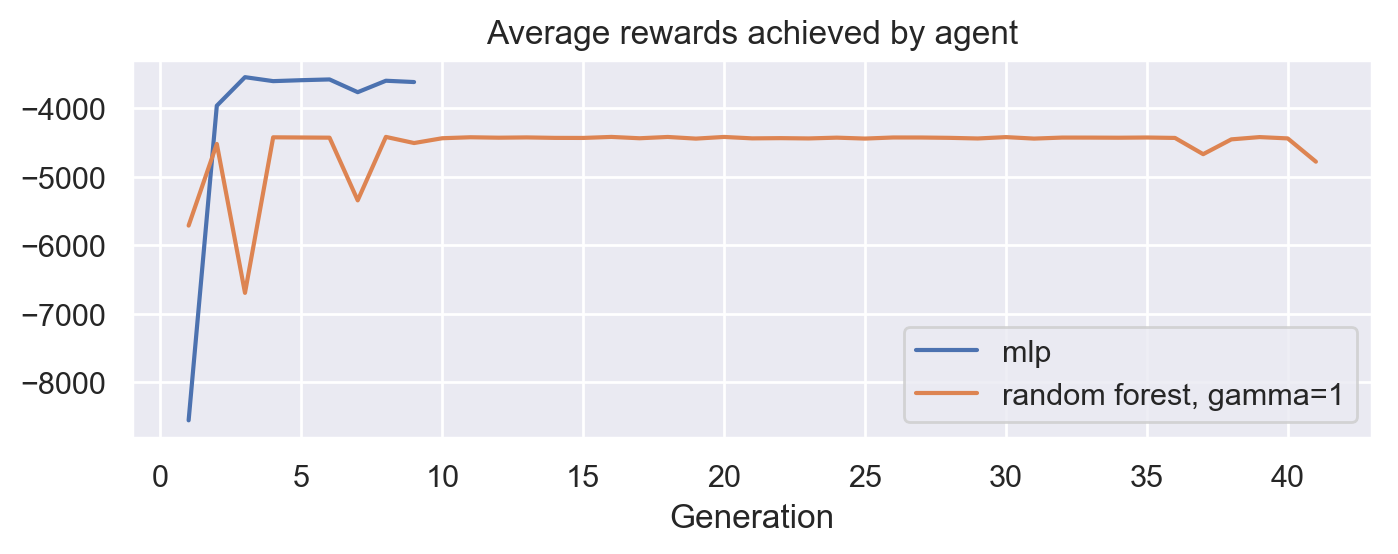
\includegraphics[width=\linewidth]{images/mlp_vs_forest_gamma_1.png}
	\caption{Here we see the performance of 40 generations trained with the random forest and 8 generations using the MLP. We chose not to train the MLP further as the time constraints were too severe and we were not seeing any improvement.}
	\label{mlp_vs_forest_gamma_1.0}
\end{figure}


%show results of initial training
%random forest too erratic - as single steps can be fatal, inaccuracies can have drastic consequences
%let train for a long time as unclear when we should see results
%present variations
%discuss changes and possible solutions - even fewer features, other machine learning methods




\section{Heins thoughts}
Tasks to be done are:
	\begin{itemize}
		\item Find a suitable \textit{state representation} to be then passed to an estimator to estimate the expected reward for each of the possible actions
		\item Find a suitable rewards in order to communicate the goals of the game to the agent
		\item Find a suitable model which estimates the expected reward for each possible action at the current state of the game.
	\end{itemize}

\subsection{State representation}
My proposal is a 2D numpy array. Each row (first index) represents a single state. Each column represents a feature. All available information is stored within each agent in the dictionary \code{self.game\_state}. What features do we store?
	\begin{itemize}
		\item For each cell:
		\begin{itemize}
			\item \textbf{Crate, wall, free \state{1,-1,0}}: The same representation is provided by \code{self.game\_state}. Only it has to be reshaped into a 1D-array. 
			\item \textbf{Cell contains agent \state{0,1}}
			\item \textbf{Cell contains opponent \state{0,1}}: This and the point above need to be stored seperately because it is possible for agent and opponent to occupy the same cell. It would just be impossible to distinguish whether a cell is occupied by just one or more opponents. But this should be a negligible issue. 
			\item \textbf{Cell contains coin \state{0,1}}
			\item \textbf{Explosion on cell}: Provided as 2D-numpy array by \code{self.game\_state}.
			\item \textbf{Danger level \state{0,\dots,4}}: How many time steps until an explosion will hit the cell.
		\end{itemize}
		\item Just once at the end of the array:
		\begin{itemize}
			\item \textbf{Current step number \state{1,\dots,400}}
			\item \textbf{Bomb action possible \state{0,1}}
			\item \textbf{Danger level:} This is a danger level for the agent. It is not necessary but provides a clearer measure of whether the agent is actually in danger. I propose to calculate this by multiplicating the danger level of each cell with the \textit{Cell contains agent} entry of each cell and then take the maximum of all the results. This way we will only get a non-zero value if the agent is on a cell with a danger level $>0$.
			\item \textbf{Reward already received in this episode}
			\item \textbf{Reward received at the end of the episode}: This one has to be added subsequently at the end of the episode to each ocurred state.
			\item \textbf{Reward gained after this state occurred:} This one is the difference of the two above. This should be our \textit{target} which we aim to maximize.
			\item \textbf{Agent touches opponent \state{0,1}}: The simple agents consider dropping a bomb if they touch an opponent. This may be a very good indicator for dropping a bomb for our model.
		\end{itemize}
	\end{itemize}
This gives us $6$ entries for each cell and $7$ entries at the end of the array. There are $17\times17$ cells in the arena. However, the cells located at the rim are always \textit{walls}. These do not need to be stored. What remains is a $15\times15$ grid. I am not sure whether we want to store cells with \textit{walls} at all, because these are always the same. They should add nothing to the state of the game.\\
Therefore we have $15\times15=225$ entries ($15\times15-7\times7=176$ if we don't store walls) plus $7$ at the end of the array for each state (time step). Storing these total $232$($183$) entries in a numpy array might produce big amounts of data. We should consider specifying the data type explicitly. However, the numpy documentation states that the data type is chosen as the minimum type required to hold the objects in the sequence.

\subsection{Rewards}
The most rewarded actions should be those which will win us the game. Those are collecting coins (1 point) and killing opponents (5 points). Therefore, I propose the same scaling between those two when rewarding them. \\
Subgoals which we consider helpful for winning should be rewarded too, but only with few points. It should be almost impossible to substitute the \textit{winning actions} (coins and killing) with \textit{helpful actions} (destroying crates). \\
I also propose a penalty of $-1$ for every action so that the agent learns to act as efficiently as possible. \\
Dying should be (beware! wordplay:) gravely punished. 
\begin{figure}[h]
	\centering
	\begin{tabular}{c|c}
		Action & Reward\\
		\toprule
		Collect coin & 100\\
		Kill opponent & 500\\
		Destroy crate & 1-2 per crate\\
		Perform action & -1\\
		Die & -500fd
	\end{tabular}
\end{figure}

\subsection{Estimator} 
I don't know much about neural networks which is why I spent most of my thoughts on how to implement this with the models we used in the exercises. Plus, I like the idea of the challenge to come up with an agent which doesn't use a neural network. \\
Since we want to estimate the expected reward of performing an action at in a given state, we need a regressor. This regressor needs to be highly flexible in order to cope with the variety of states. I guess the most flexible regressor we used would be a \textit{Random Forest Regressor}. On the one hand, this one would need tons of learning data but on the other hand, which proper regressor doesn't?\\
This means, we would plug the data of the states and the received rewards into the model and get an estimate of what reward we could expect for what action. Since we need to distinguish between the six possible actions, we need six Random Forests. One for each action. Each forest trained only with the states after which the respective action was performed. This also means that we need to store all data in six different set for six possible actions or store the action performed afterwards in the \textit{state vector}.

\subsection{Learning algorithm}
I propose to use the Max-Boltzmann (MB) method as described in \cite{paper} or something similar. It is mostly a $\epsilon$-greedy algorithm. But when it decides to explore, it doesn't choose randomly among the remaining actions but assigns probabilities corresponding to the value (expected reward) of the remaining action. This way, exploration is not just random but more targeted.\par

There is no point in letting the agent learn after every single episode. In the long run those learning interruptions will cost us a lot of time. Plus, it is very unlikely that the next episodes are similar to the one before which means that the learning will most likely not be applied in the subsequent episodes. Thus, the learning process itself should be divided into learning intervals of many episodes, say 100 to 1000, maybe even 10000 episodes, given the number of possible states. While we're already using the term \textit{episodes}, let's call those learning intervals \textit{seasons}.\par
I propose the following procedure:
\begin{enumerate}
	\item Use the provided simple agent as our agent to play the first season. I would use the MB algorithm already in the first episode. This already gives us the possibility of exploration which I consider as important since the simple agent is fully determined and hard coded.
	\item Use the data of the first season to train our model. 
	\item From now on, let the agent rely only on the predictions of our model. Create data, explore according to the MB algorithm. 
	\item Use the data of all former seasons to again train our model.
	\item Repeat the two former steps.
\end{enumerate}
The simple agents should be good sparring partners to start with. They are very good at avoiding bombs but sometimes lack the ability to collect coins. We might improve this ability in the simple agent code to get better starting conditions. Maybe by automatically decreasing the distance (and thus increasing importance) of coins.
\subsection{Necessary functions}
Some functions that need to be implemented in order to prepare everything:
\begin{itemize}
	\item Calculate danger levels of each cell
	\item Insert \textit{coins} into \textit{state vector}
	\item Insert \textit{opponents} into \textit{state vector}
	\item Insert \textit{self} into \textit{state vector}
\end{itemize}
We need to decide what structure the \textit{state vector} should have. There are two ways:
\begin{enumerate}
	\item All features of a concerning cell (coin, opponent, self, danger level,...) subsequently. The all features of the next cell and so on \dots
	\item All data of one feature (e.g. coin) for all cells, then all data of the next feature for all cells and so on \dots
\end{enumerate}
In both cases, the functions that insert the values into the array should make use of the slicing possibilities of numpy arrays (e.g. \code{x[starting point:end point:stepsize]}). In the first case, only every sixth entry represents the same feature. In the second case, the first hundred entries represent only one feature for different cells.

\section{Karls thoughts}

How this project can be approached:
	\begin{itemize}
		\item Neural Network approach \textit{vs.} Classical Machine learning approach
		\begin{itemize}
			\item Supervised learning \textit{vs.} Reinforcement learning \textit{vs.} Unsupervised learning
			\item Feature selection to determine relevant information the agent should "see" and learn from
		\end{itemize}
		\item Data management for training - not necessary as we will be collecting all the relevant data while training rather than using a large pre-compiled dataset
	\end{itemize}

As we do not have access to more than our own laptops which can not be classed as high performance systems with low end dedicated GPUs training neural networks may be impractical and time consuming.

\subsection{Neural Networks}
As we didn't cover neural networks in the lecture but are allowed to apply them to this Project I explored it as an option despite knowing we are likely to select the classical approach.
Some algorithms that are worth exploring are:
	\begin{itemize}
		\item Supervised learning:
		\begin{itemize}
			\item Gradient descent involves forming a continuous error function using rewards to minimize
		\end{itemize}
		\item Reinforcement learning:
		\begin{itemize}
			\item Q-Learning (as covered in lectures)
			\item Genetic Algorithm:
			\begin{itemize}
				\item Training occurs through improvements from generation to generation by improving the strength and bias values for the edges of the neural network (stored in a 1D array). Each generation has a set number of instances that follow a variation of the previous generations values. To decide which of the instances in the previous generation had the best strength and bias values a scoring system must be created based on the performance of each instance.
				\item Outputs are predetermined as 5 movement options (up, down, left, right, stand still) and the Bomb placement option
				\item Factors to be decided on:
				\begin{itemize}
					\item Inputs e.g. \textit{weighted score of distance to enemies/crates/coins/bombs}
					\item Number of hidden layers and nodes (not sure how this is done yet)
					\item Method for genetic variation e.g. \textit{ranking by score and weighting the likelihood for this process to be selected, random selection}. This is the exploitation aspect. Some values however should be randomly changed or multiple arrays crossed together (like nature) to increase the likelihood of finding the global minimum rather than local (exploration.
				\end{itemize}
			\end{itemize}
		\end{itemize}
	\end{itemize}		

\subsection{Classical approach}
We could use Q-learning to train a $\epsilon$-greedy agent. We want to find the optimal policy \textbf{Q} to solve the game.

Here its important to identify the 2 sets of attributes that contribute to decision making, \textbf{state} and \textbf{action}. The state will be input to decision making function to determine the action, the features that describe the state however must first be decided on.
To reduce runtime it may be advantageous to perform a dimension reduction if it becomes clear that some features for example the states of the cells outside of a 5x5 radius around the agent have very little impact on the decision. This could be particularly important in the early tests before the final train to reduce training time required when for example testing various reward value boundaries.

\subsubsection{State appraisal}
Before a decision can be reached as to the next action clearly the state of the board must first be assessed. With an almost infinite number of possible inputs possible it is important to have as few and as relevant features as possible.

Ideas to test/discuss:
\begin{itemize}
	\item Are all accessible fields relevant
	\item Is it possible to approximate the state with knowledge about only the non-empty fields. In extreme cases this can be 2 (final 2 agents) or 176 (all fields occupied, although this is a stalemate) so this is likely not constructive.
	\item How should the distances to other agents or items be stored? Possibilities include:
	\begin{itemize}
	\item The route that could be taken
	\item Only the coordinates
	\item The number of moves required to move the the desired opponent or coins field and the direction. Here the shorter route could also be through boxes and therefore include bomb wait times
	\end{itemize}	 
	\item Should any previous states have a weighted input? - probably not, could be useful in some edge cases maybe?
\end{itemize}

\subsubsection{Rewards}
Naively we want to positively reinforce proactive, safe actions and negatively reinforce hazardous or even fatal actions so we should set our rewards based on this structure. This may however not always lead to the optimal solution as there are some situations where a sacrifice can lead to a greater boon in later steps e.g. \textit{queen sacrifice for checkmate in chess}.

We have essentially 3 choices for how to issue rewards:
\begin{itemize}
	\item Updating Q after each episode:
	\begin{itemize}
		\item This leads to faster training times as the entire episode can play out without interruptions, however each episode leads to slower improvement as the Agent can only perceive the results of all decisions made during the episode.
	\end{itemize}

	\item Stepwise Q updates:
	\begin{itemize}
		\item Very slow episodes (opposite of episodic updates above)
		\item Ultimately it will depend on how we set our rewards, whether a movement to a cell should be rewarded based on proximity to other agents/bombs or coins and how we allow these factors to influence the positivity or negativity of an action. I.e. A step towards a coin that is also a step into an exploding bomb should lead to a negative reward.
		\item This would allow for punishment for the repetition of actions, such as the movement to a previously occupied square which may be undesirable and therefore punished with a small negative value
		\item Decisions that are not allowed in certain situations such as movement into a wall/crate should also be punished harshly
	\end{itemize}			
	\item N-step Q updates: see above every N steps
\end{itemize}

Importantly the values for rewards should be small to ensure numerical stability in later operations

\subsubsection{Exploration vs. Exploitation}
\begin{itemize}
	\item e-greedy policy 
	
	[[learn to Tex maths]]
	\item soft max policy to max the "Temperature" S over time
	
	[[learn to Tex maths]]
\end{itemize}


\section{Karls observations}

These are just notes to document stages of development and note questions that arise.
\subsection{The state matrix}
\begin{itemize}
	\item How should a bombs presence be documented in the 'state' matrix? 
	\item Should a bomb timer be the input?
	\item Is there any value in including the fields that have an explosion in them? 
	I can't think of a situation in which this would be relevant to making a decision for the next action.
\end{itemize}

%%%%%%%%%%%%%%%%%%%%%%%%%%%%%%%%%%%%%%%%%%%%%%%%%%%%%%%%%%%%%%%%%%%%%%%%%%%%%%%%%%%%%%%%%
\begin{thebibliography}{111}
   

%if the "underfill \hbox" warning bothers you uncomment the following line
%\raggedright


\bibitem{RL_intro}
Richard S. Sutton, Andrew G. Barto (2018)\\
\textit{Reinforcement Learning: An Introduction}\\
Available at: http://incompleteideas.net/book/bookdraft2018jan1.pdf

\bibitem{paper}
Joseph Groot Kormelink, Madalina M. Drugan and Marco A. Wiering (ICAART 2018)\\
\textit{Exploration Methods for Connectionist Q-Learning in Bomberman}\\
Available at: https://bit.ly/2GReSxQ
\end{thebibliography}
\end{document}

%This template was created by Roza Aceska.